\cotefile{10}
\scanpage{77}
\mspage{76}
quotient of $\handwritten{\overline}{\handwritten{\underline}{Q}}^{\handwritten{*}}$ by the subgroup of units, hence canonically isomorphic to $\handwritten{\underline}{Q}$, by the isomorphism
\[
\handwritten{\overline}{\handwritten{\underline}{Q}}^{\handwritten{*}}/\text{units}\handwritten{\longrightarrow}\handwritten{\underline}{Q}
\]
given by the p-adic valuation $v_p$, normalized by the condition
\[
v_p(p)=1\quad .
\]
\unsure{\rlap{A}The|A|The} action of $\deleted{\unsure{\pi|\Pi}_1(\underline{\unsure{\rlap{F}K|K|F|k}}}$ $\operatorname{Gal}(\handwritten{\overline}{\handwritten{\underline}{Q}}_p/\handwritten{\underline}{Q}_p)$ on this quotient group $Q$ is trivial\unsure{\rlap{i}e|\.{e}|e}, so that $H$ is \handwritten{\uline}{diagonalizable} with character group $\handwritten{\underline}{Q}$:
\[
H=D(\handwritten{\underline}{Q})\quad .
\]
The Tate augmentation of $G$ corresponds to the homomorphism
\[
\handwritten{\underline}{Z}\handwritten{\longrightarrow}\handwritten{\overline}{\handwritten{\underline}{Q}}^{\handwritten{*}},\quad 1\handwritten{\longmapsto}p\quad ,
\]
and the augmentation induced on $H$ corresponds to the canonical \handwritten{\uline}{inclusion}
\[
\handwritten{\underline}{Z}\handwritten{\lhook\joinrel\longrightarrow}\handwritten{\underline}{Q}
\]
(thanks to our choice of the valuation \handwritten{\uline}{normalized} as indicated\unsure{\rlap{i}e|\.{e}|e}).

\unsure{\rlap{8}B|B|8}.2. We must now make explicit the homomorphism of \unsure{\rlap{e}g|g}erbes
\[
\handwritten{\text{(8\unsure{,|.}2.1)}}\qquad\handwritten{i:}\ \handwritten{\underline}{G}(\handwritten{\underline}{F}_p)\handwritten{\longrightarrow}\handwritten{\underline{\pi}}_p(\handwritten{\underline}{F}_p)

\]
corresponding to the inclusion
\[
i:\quad \handwritten{\underline}{Q}_p\text{-constructible sheaves}\handwritten{\lhook\joinrel\longrightarrow}\operatorname{Fcriso}(\handwritten{\underline}{F}_p)
\]
of 5.2. We have seen that the essential image is exactly equal to the \inserted{full} subcategory \handwritten{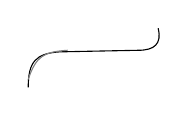
\begin{tikzpicture}[baseline=0cm,x=1cm,y=1cm]\draw[thin] (0,-.35)..controls (0,-.02) and (.1,.08)..(.4,.1)--(1.4,.12)..controls (1.6,.12) and (1.7,.2)..(1.65,.4);\draw[gray,thin] (0,-.25)..controls (.1,.05) and (.2,.1)..(.5,.12);\end{tikzpicture}} $j(\handwritten{\underline}{Q}_p\text{-constructible sheaves})$, \deleted{which is} so that $i$ is identified with a\deleted{functor} $\handwritten{\unsure{\mathrel{
\begin{tikzpicture}[baseline=-.12cm,x=1cm,y=1cm]\draw[thick] (.05,0) ellipse (.22 and .3);\draw[thick] (-.1,-.2)--(.19,.2);\draw[thick] (-.1,.2)--(.19,-.2);\draw[thin] (-.22,-.23)--(-.22,.2);\draw[thin] (-.31,.2)--(-.17,.2);\draw[thin] (-.31,-.23)--(.22,-.23);\end{tikzpicture}}}}$-equivalence of the category of constructible $\handwritten{\underline}{Q}_p$-sheaves with itself. We then find that the corresponding homomorphism on the bands $\deleted{\unsure{H\ H|H\to H}}$ $G'\handwritten{\longrightarrow}G'$ is the identity, \deleted{and that} so that $i$ is defined by a torsor under $G'$, and that this torsor under $G'$ can be described as follows (could have gone at the end of 7, in the case of an arbitrary $k$ ...). We have a canonical homomorphism
\[
\handwritten{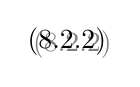
\begin{tikzpicture}[baseline=(dark.base),x=1cm,y=1cm]\node[gray,inner sep=0pt] at (.07,-.04) {$(8.2.2)$};\node[inner sep=0pt] (dark) at (0,0) {$(8.2.2)$};\end{tikzpicture}}\qquad\handwritten{\pi}_1(\handwritten{\underline}{F}_p^{\deleted{\handwritten{\unsure{*|\times}}}})=\overset{\deleted{\handwritten{\unsure{2|*|\times}}}}{\handwritten{\hat}{\handwritten{\underline}{Z}}}\handwritten{\longrightarrow}G'(\handwritten{\underline}{Q}_p),\quad \handwritten{\text{i.e. }(\pi_1(\underline{F}_p))_{\mathbb{Q}_p}\longrightarrow G'}

\]
whence a \deleted{homomorphi} functor
\[
\text{torsors}^{\deleted{\underline{Q}_p\text{-}}}\text{ under }(\handwritten{\hat}{\handwritten{\underline}{Z}})_{\handwritten{\underline}{Q}_p}\handwritten{\longrightarrow}\text{torsors under }G'\ \deleted{\handwritten{\unsure{\xi|\varepsilon|,|.}}}
\]
